%%%%%%%%%%%%%%%%%%%%%%%%%%%%%%%%%%%%%%%%%%%%%%%%%%%
\fe{\section{Présentation}}{\section{Presentation}}
\label{presentation}
%%%%%%%%%%%%%%%%%%%%%%%%%%%%%%%%%%%%%%%%%%%%%%%%%%%

\begin{frame}{\fe{Cast3M, quid ?}{What is Cast3M?}}
  \begin{center}
    \fe{Logiciel de simulation utilisant la \g{méthode des éléments finis} en \g{mécanique/thermique} des \g{structures} et des \g{fluides}}
       {A simulation software using the \g{finite element method} in \g{thermal and mechanical} analysis of \g{structures} and \g{fluids}}\pause
  \end{center}
  \begin{itemize}
    \item \fe{Résolution d'\g{équations aux dérivées partielles}}
             {\g{Partial differential equations} solver}\pause
    \item \fe{\g{Système complet} : solveur, pré/post-processeur, visualisation, import/export des données\dots}
             {\g{Complete software}: solver, pre-processing and post-processing, visualization, reading/writing data\dots}\\~\\
    \begin{center}
      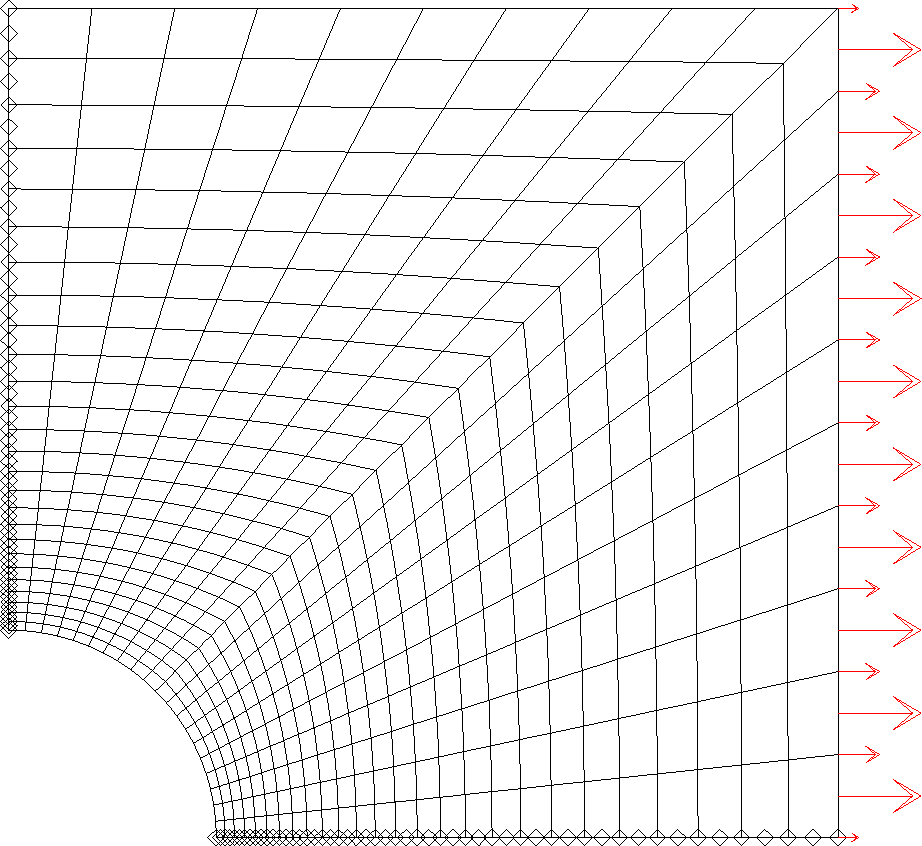
\includegraphics[height=0.25\textheight]{images/plaque.1} \:
      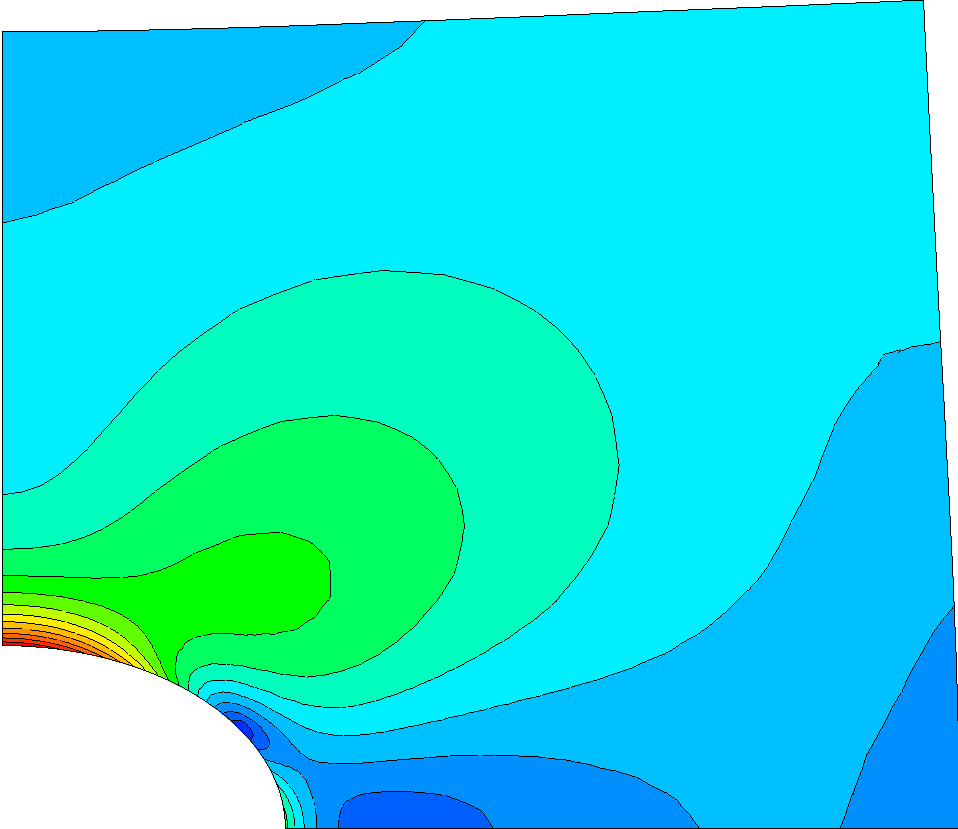
\includegraphics[height=0.25\textheight]{images/plaque.2} \:
      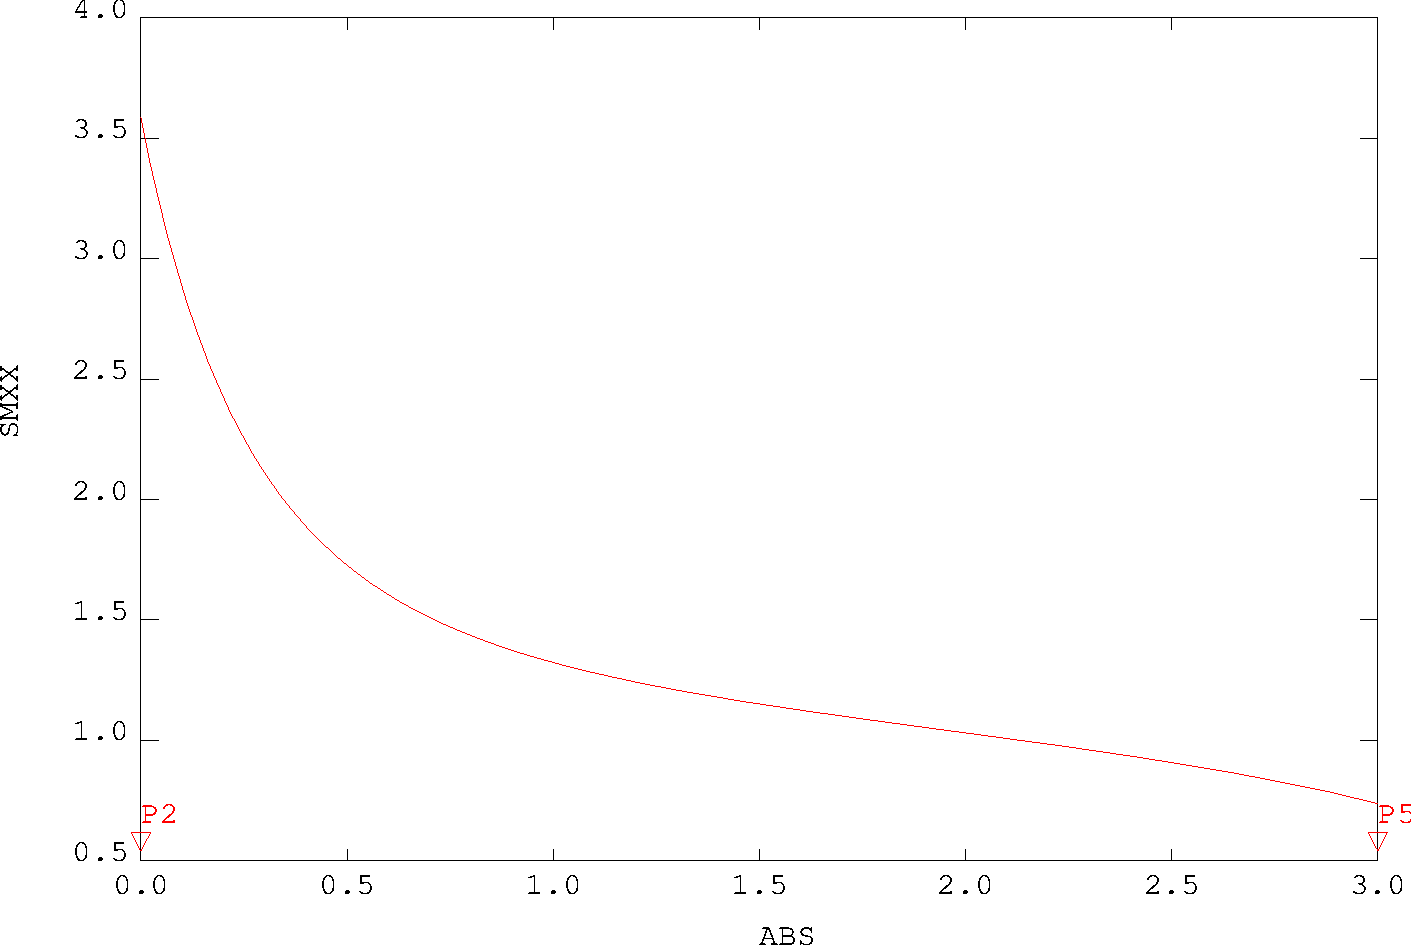
\includegraphics[height=0.25\textheight]{images/plaque.3}
    \end{center}\pause
    \item \fe{Basé sur un langage de commande : \g{Gibiane} (orienté objet)}
             {Based on a programming language: \g{Gibiane} (objet-oriented)}\\
  \end{itemize}
\end{frame}

\begin{frame}{\fe{Nombreux domaines d'application}{Wide range of applications}}
  \small
  \begin{itemize}
    \item<1->\fe{\g{Mécanique des structures}}{\g{Structural mechanics}}\\
    \footnotesize
    \fe{\red{Quasi-statique} (non linéarités matériau, géométrie, conditions limites)}
       {\red{Quasi-static} (non linear behavior, geometry, boundary conditions)}\\
    \onslide<1>{
      \begin{textblock*}{4cm}(0cm,0cm)
        \begin{center}
          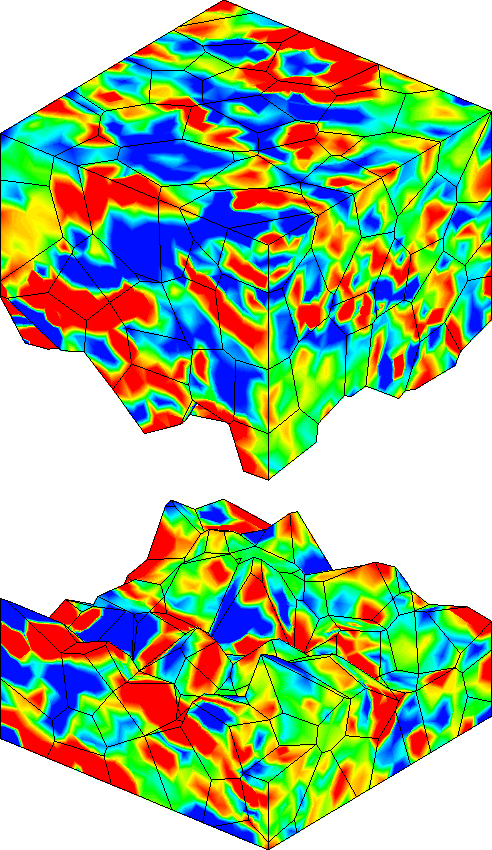
\includegraphics[height=0.4\textheight]{images/polycristal}\\
          \tiny{\fe{\emph{Microstructure : agrégat polycristallin}}{\emph{Microstructure: polycrystalline aggregate}}}
        \end{center}
      \end{textblock*}
      \begin{textblock*}{4cm}(3.4cm,0.8cm)
        \begin{center}
          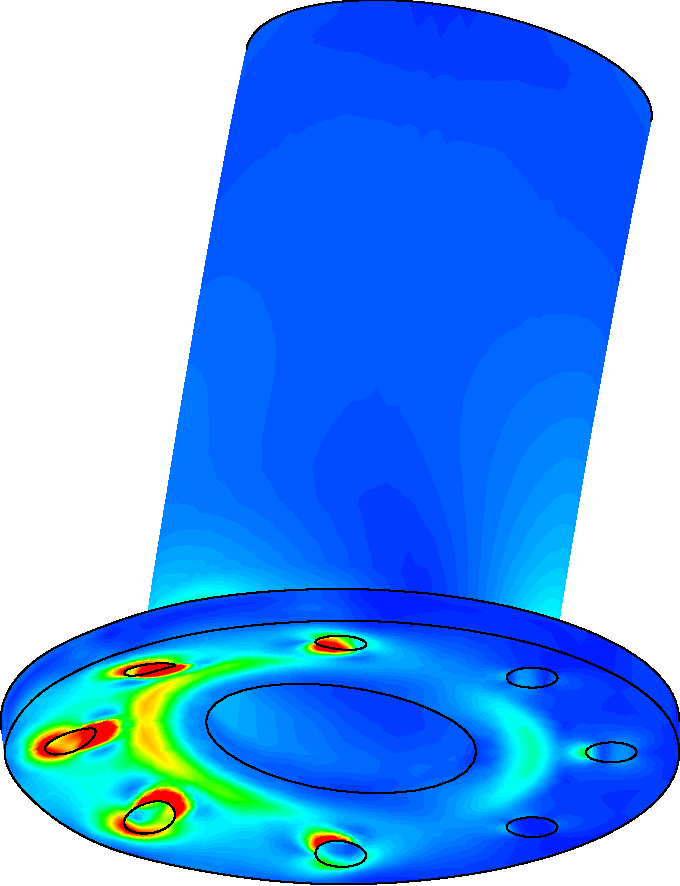
\includegraphics[height=0.4\textheight]{images/tube}\\
          \tiny{\fe{\emph{Composant : liaison d'un tube}}{\emph{Component: connection on a tube}}}
        \end{center}
      \end{textblock*}
      \begin{textblock*}{5cm}(7.2cm,1.6cm)
        \begin{center}
          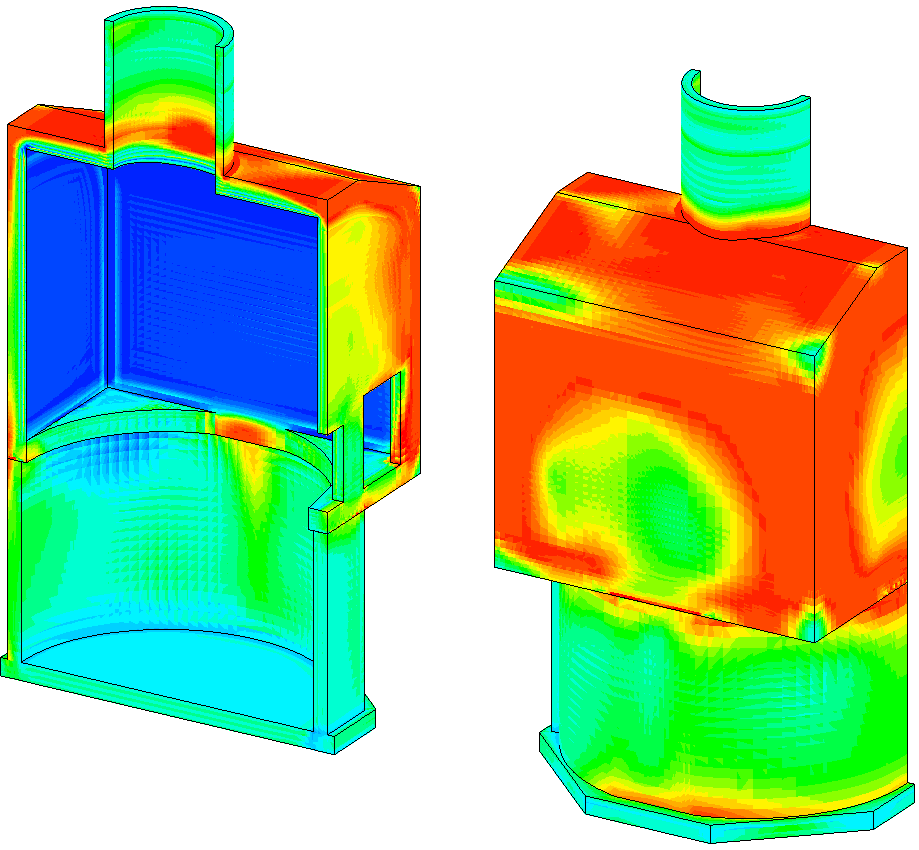
\includegraphics[height=0.4\textheight]{images/galatee}\\
          \tiny{\fe{\emph{Batiment en béton armé (S. Durand)}}{\emph{Reinforced concrete building (S. Durand)}}}
        \end{center}
      \end{textblock*}
      }
    \onslide<2->\fe{\orange{Contact/frottement}, \green{Flambage}}
                    {\orange{Contact/friction}, \green{Buckling}}\\
    \onslide<2>{
      \begin{textblock*}{10cm}(1cm,0.2cm)
        \begin{center}
          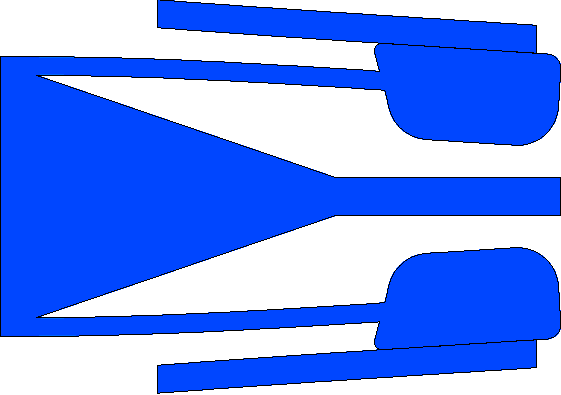
\includegraphics[height=0.25\textheight]{images/sac_a_dos.15}
          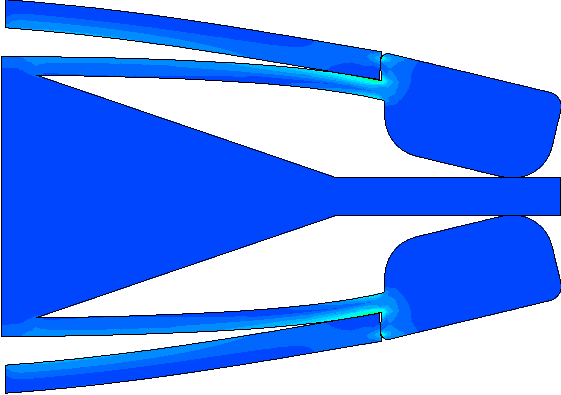
\includegraphics[height=0.25\textheight]{images/sac_a_dos.32}
          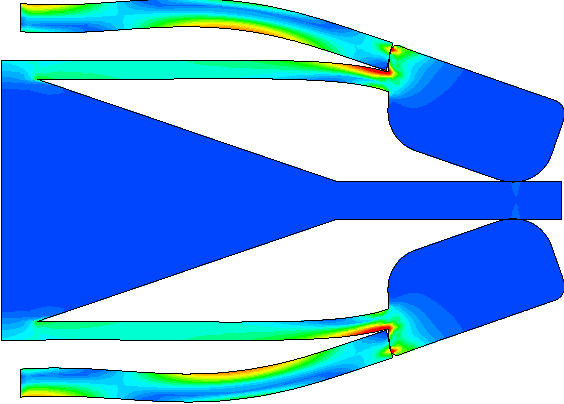
\includegraphics[height=0.25\textheight]{images/sac_a_dos.41}\\
          \tiny{\fe{\emph{Attachement d'un clip (contact + plasticité)}}{\emph{Locking a clip buckle (contact + plasticity)}}}
        \end{center}
      \end{textblock*}
      }
    \onslide<3->\fe{\blue{Dynamique} (temporelle, modale, interaction fluide structure)}
                   {\blue{Dynamic} (temporal, modal, fluid structure interaction)}\\
    \onslide<3>{
      \begin{textblock*}{10cm}(1cm,0.2cm)
        \begin{center}
          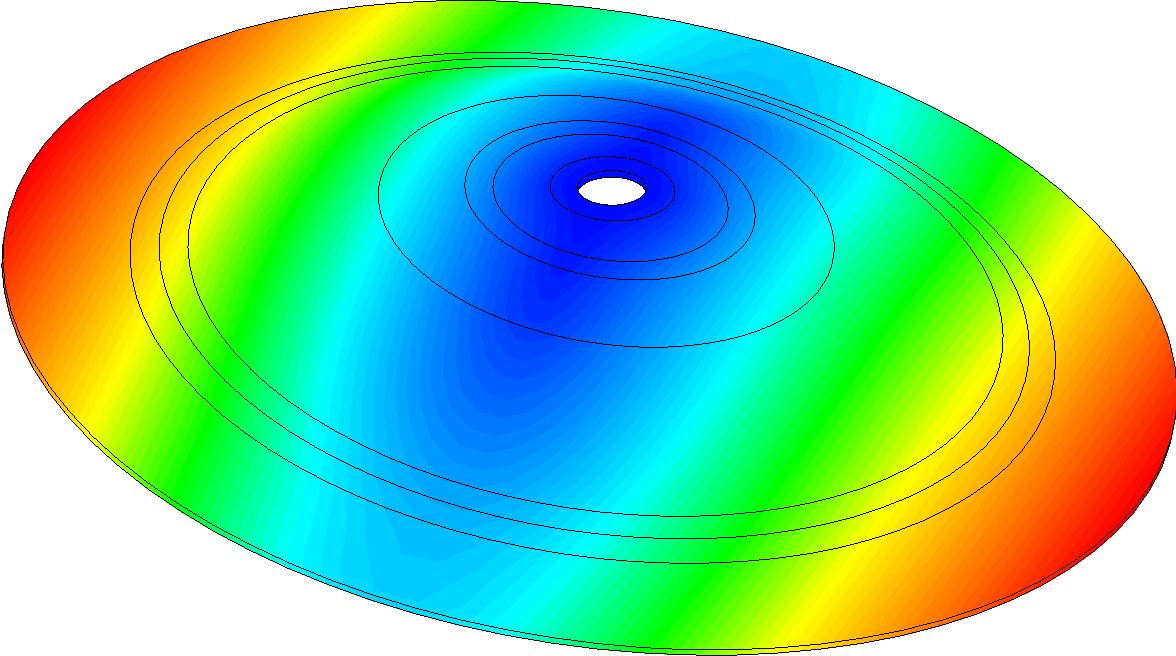
\includegraphics[height=0.2\textheight]{images/cymbale_mode_1}
          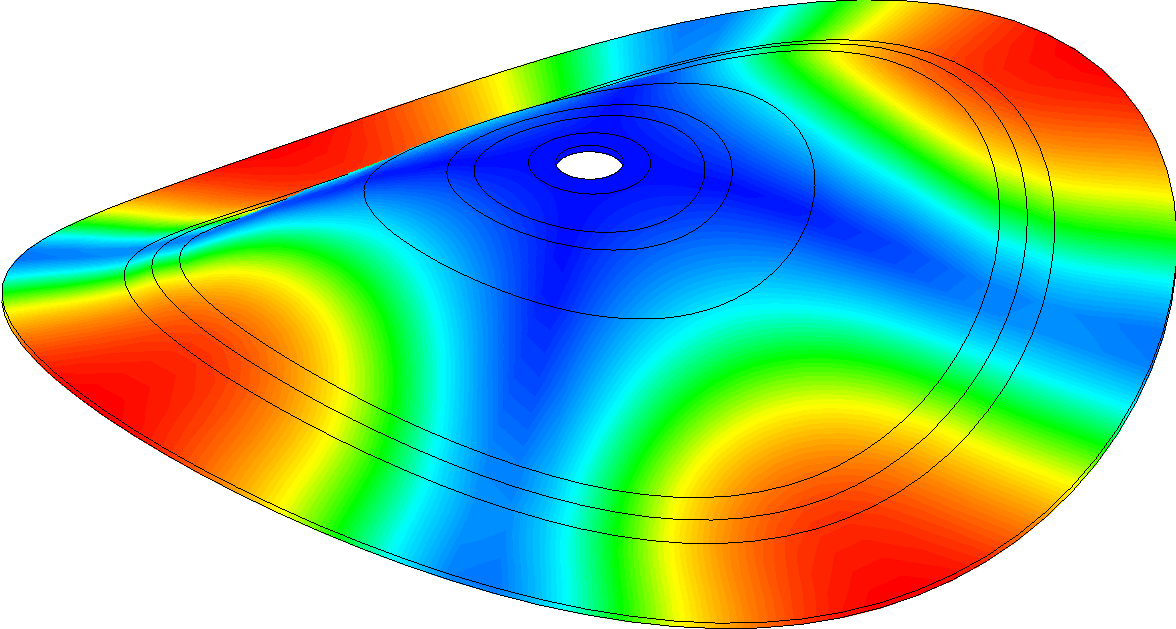
\includegraphics[height=0.2\textheight]{images/cymbale_mode_2}
          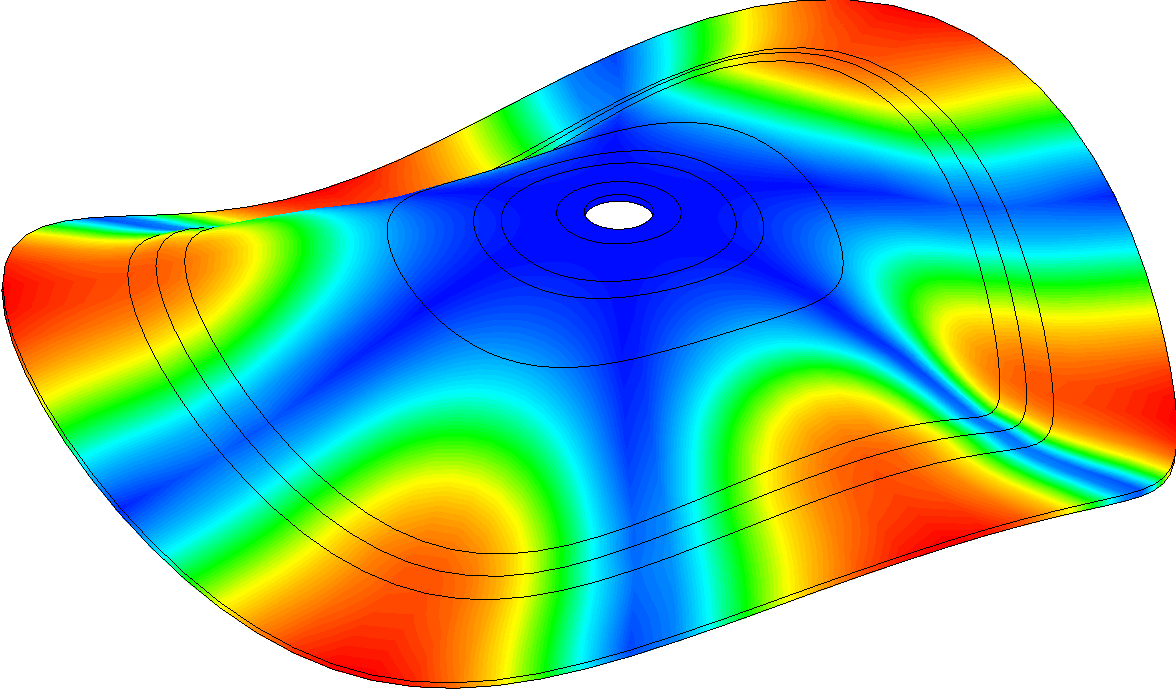
\includegraphics[height=0.2\textheight]{images/cymbale_mode_4}\\
          \tiny{\fe{\emph{Premiers modes propres d'une cymbale}}{\emph{First eigenmodes of a cymbal}}}
        \end{center}
      \end{textblock*}
      }
    \onslide<4->{\fe{\violet{Rupture} (XFEM, propagation dynamique, zones cohésives)}
                    {\violet{Fracture} (XFEM, dynamic propagation, cohesive zones models)}}\\
    \only<4>{
      \begin{textblock*}{11cm}(1cm,0cm)
        \begin{center}
          \if \animation 1
            \animategraphics[controls,loop,poster=last,height=4cm]{3}{images/rupture_ct/rupture_ct_}{1}{8}
            \animategraphics[controls,loop,poster=last,height=4cm]{3}{images/rupture_ct/rupture_ct_detail_}{1}{8}\\
          \else
            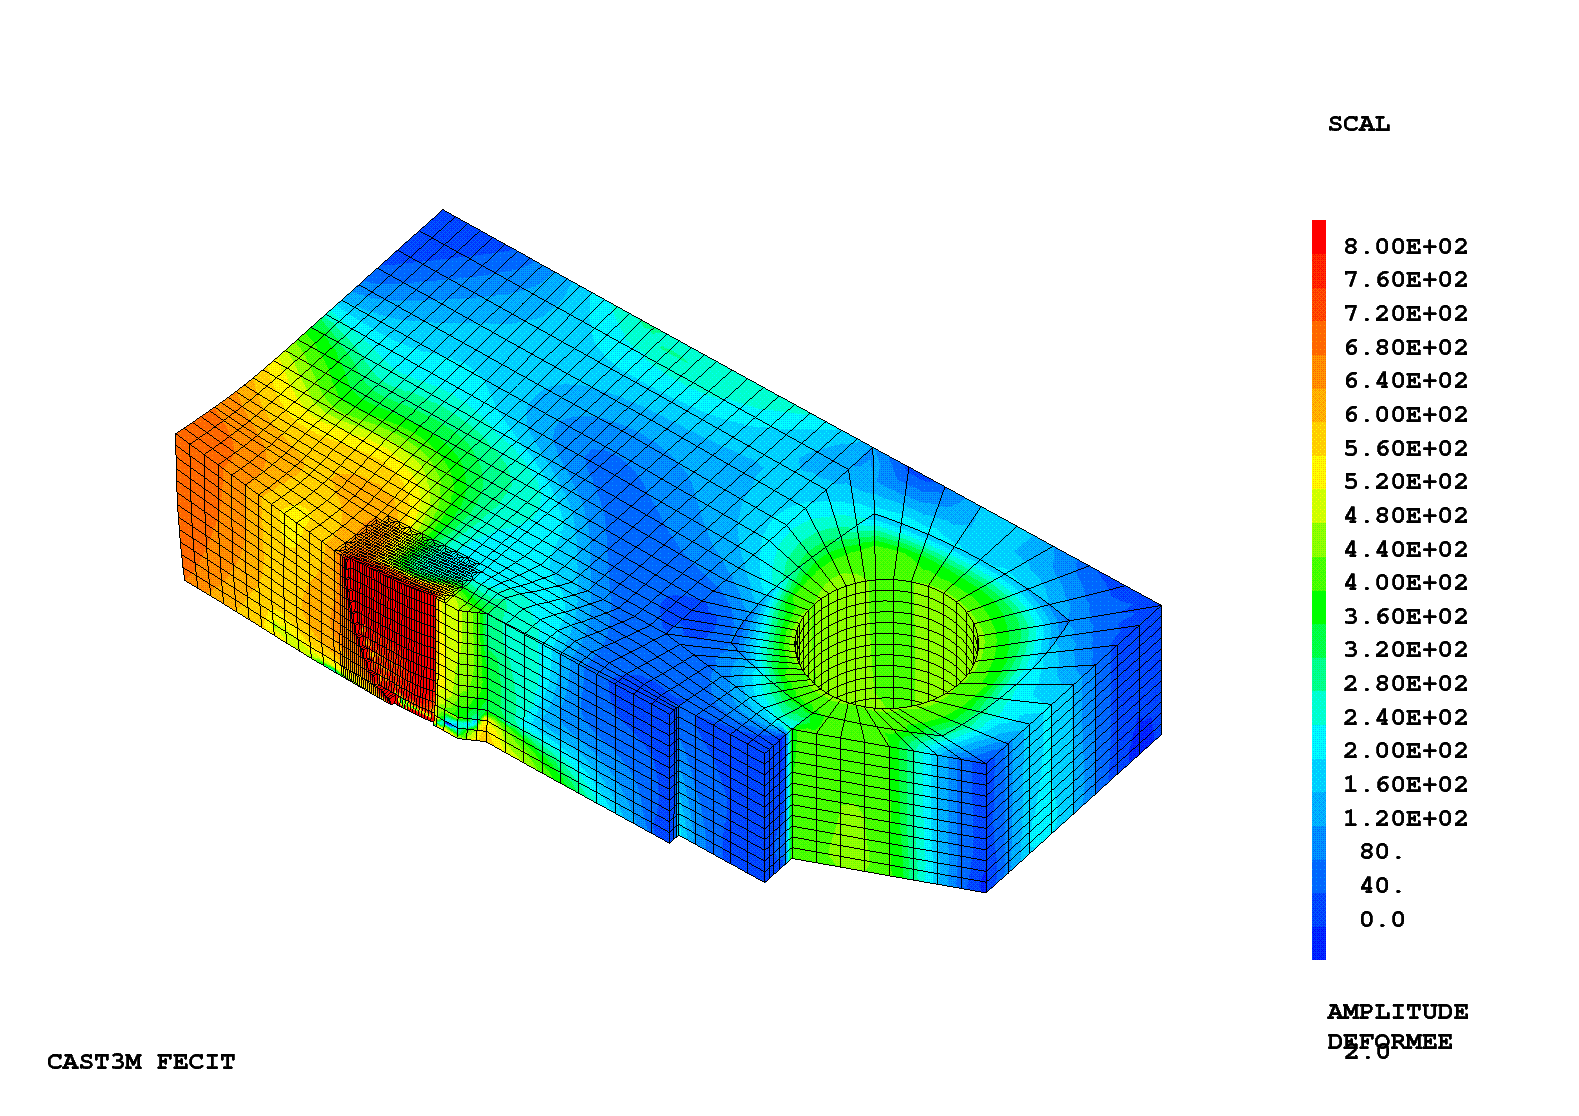
\includegraphics[height=4cm]{images/rupture_ct/rupture_ct_8}
            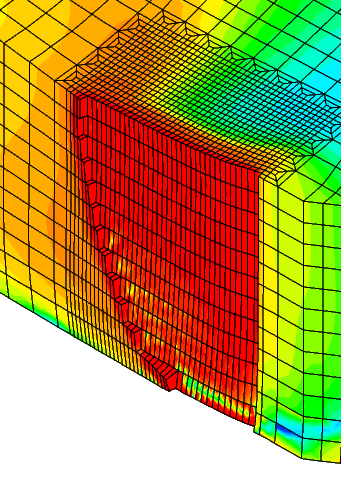
\includegraphics[height=4cm]{images/rupture_ct/rupture_ct_detail_8}\\
          \fi
          \tiny{\fe{\emph{Rupture d'éprouvette CT, plasticité/endommagement, suppression d'éléments lors du calcul (S. Kebiri)}}
                   {\emph{Fracture of a CT sepcimen, plasticity/dammage, elements removal during computation (S. Kebiri)}}}
        \end{center}
      \end{textblock*}
      }
    \small
    \item<5->\fe{\g{Thermique}}{\g{Thermal analysis}}\\
    \footnotesize
    \onslide<5->{\fe{Conduction, convection, advection, rayonnement, changement de phase}
                    {Conduction, convection, advection, radiation, phase transition}}\\
    \onslide<5>{
      \begin{textblock*}{10cm}(1cm,0.1cm)
        \begin{center}
          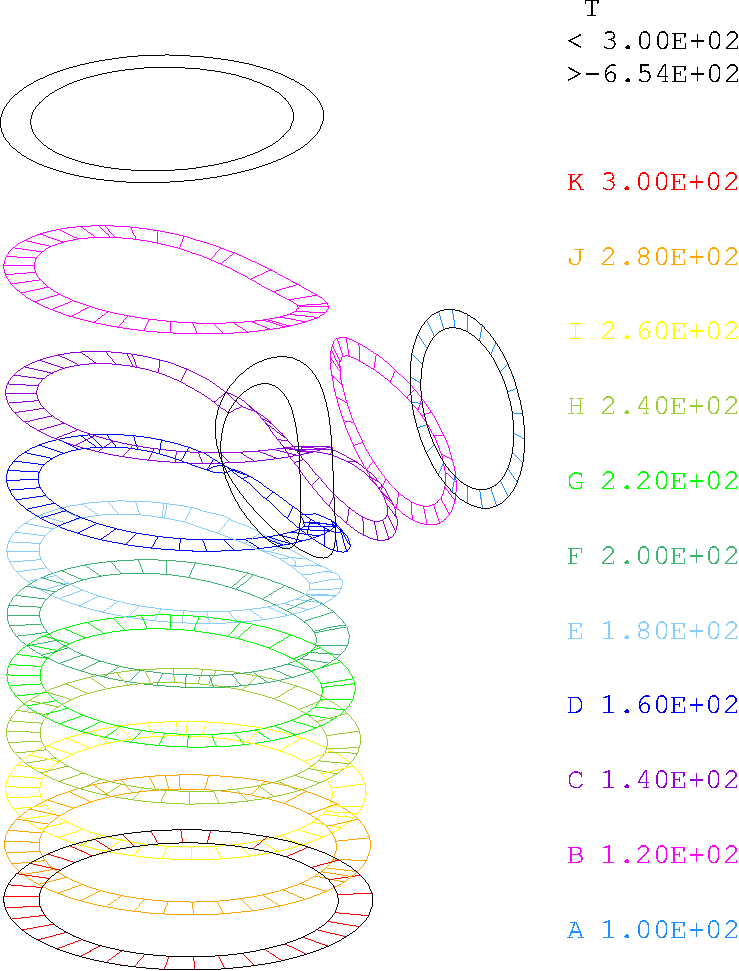
\includegraphics[height=0.4\textheight]{images/te_temperature}\hspace{1cm}
          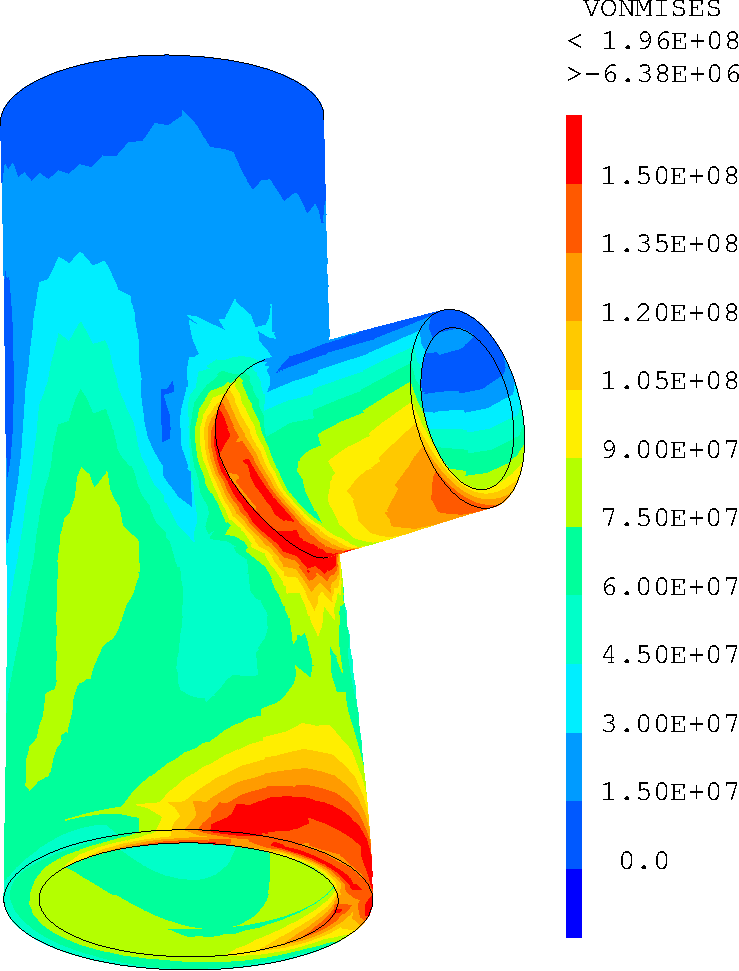
\includegraphics[height=0.4\textheight]{images/te_sigma}\\
          \tiny{\fe{\emph{Thermo mécanique d'un té de tuyauterie}}{\emph{Thermo mechanical analysis of a pipe tee}}}
        \end{center}
      \end{textblock*}
      }
    \small
    \item<6-> \fe{\g{Mécanique des fluides}}{\g{Fluid mechanics}}
    \item<6-> \fe{\g{Diffusion} multi espèces (loi de Fick)}{Multi species \g{diffusion} (Fick's law)}\\
    \item<6-> \fe{Fabrication additive, Métallurgie}{Additive manufacturing, Metallurgy}\\
    \footnotesize
    \only<6>{
      \begin{textblock*}{7cm}(5.7cm,-2cm)
        \begin{center}
          \if \animation 1
            \animategraphics[controls,loop,poster=last,width=5cm]{20}{images/fab_add/fab_add_}{001}{397}\\
          \else
            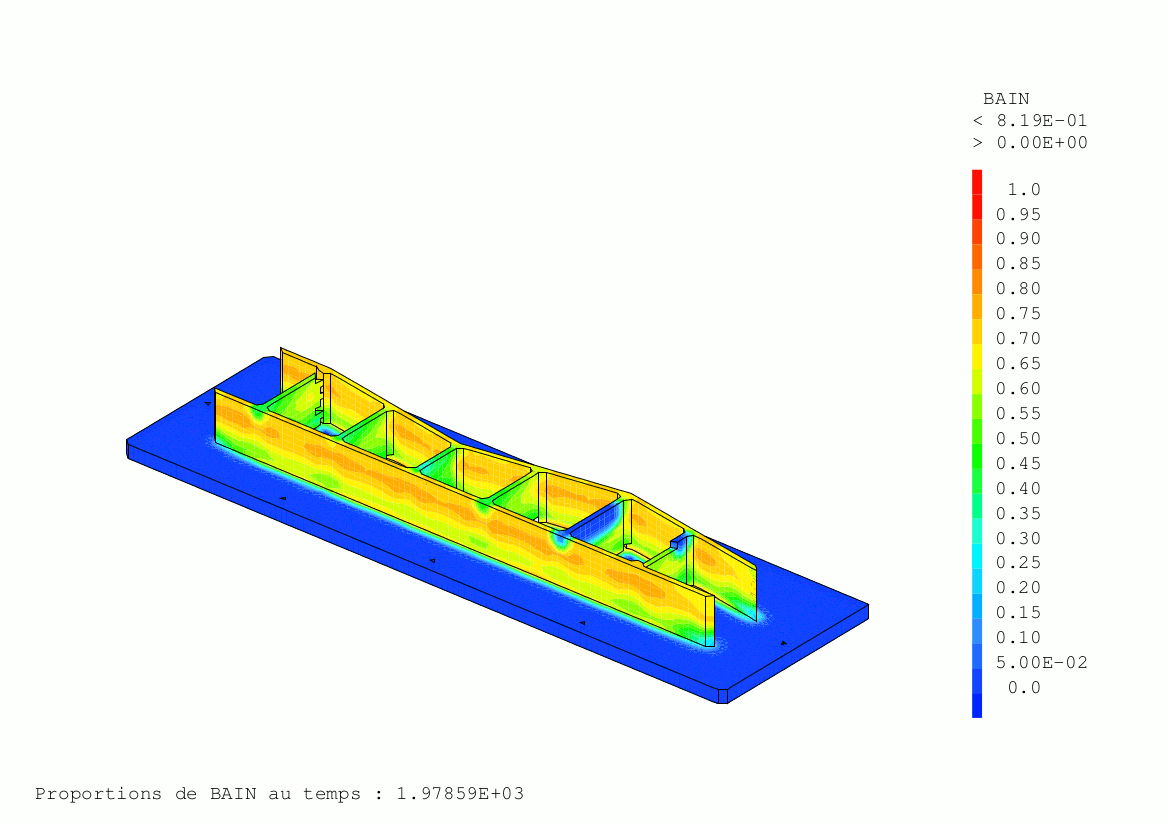
\includegraphics[width=5cm]{images/fab_add/fab_add_397}\\
          \fi
          \tiny{\fe{\emph{Proportion de bainite lors d'une fabrication additive (C. Berthinier)}}
                   {\emph{Proportion of bainite during the additive manufacturing (C. Berthinier)}}}
        \end{center}
      \end{textblock*}
      }
    \onslide<7>{
      \begin{textblock*}{5cm}(6.5cm,-1.5cm)
        \begin{center}
          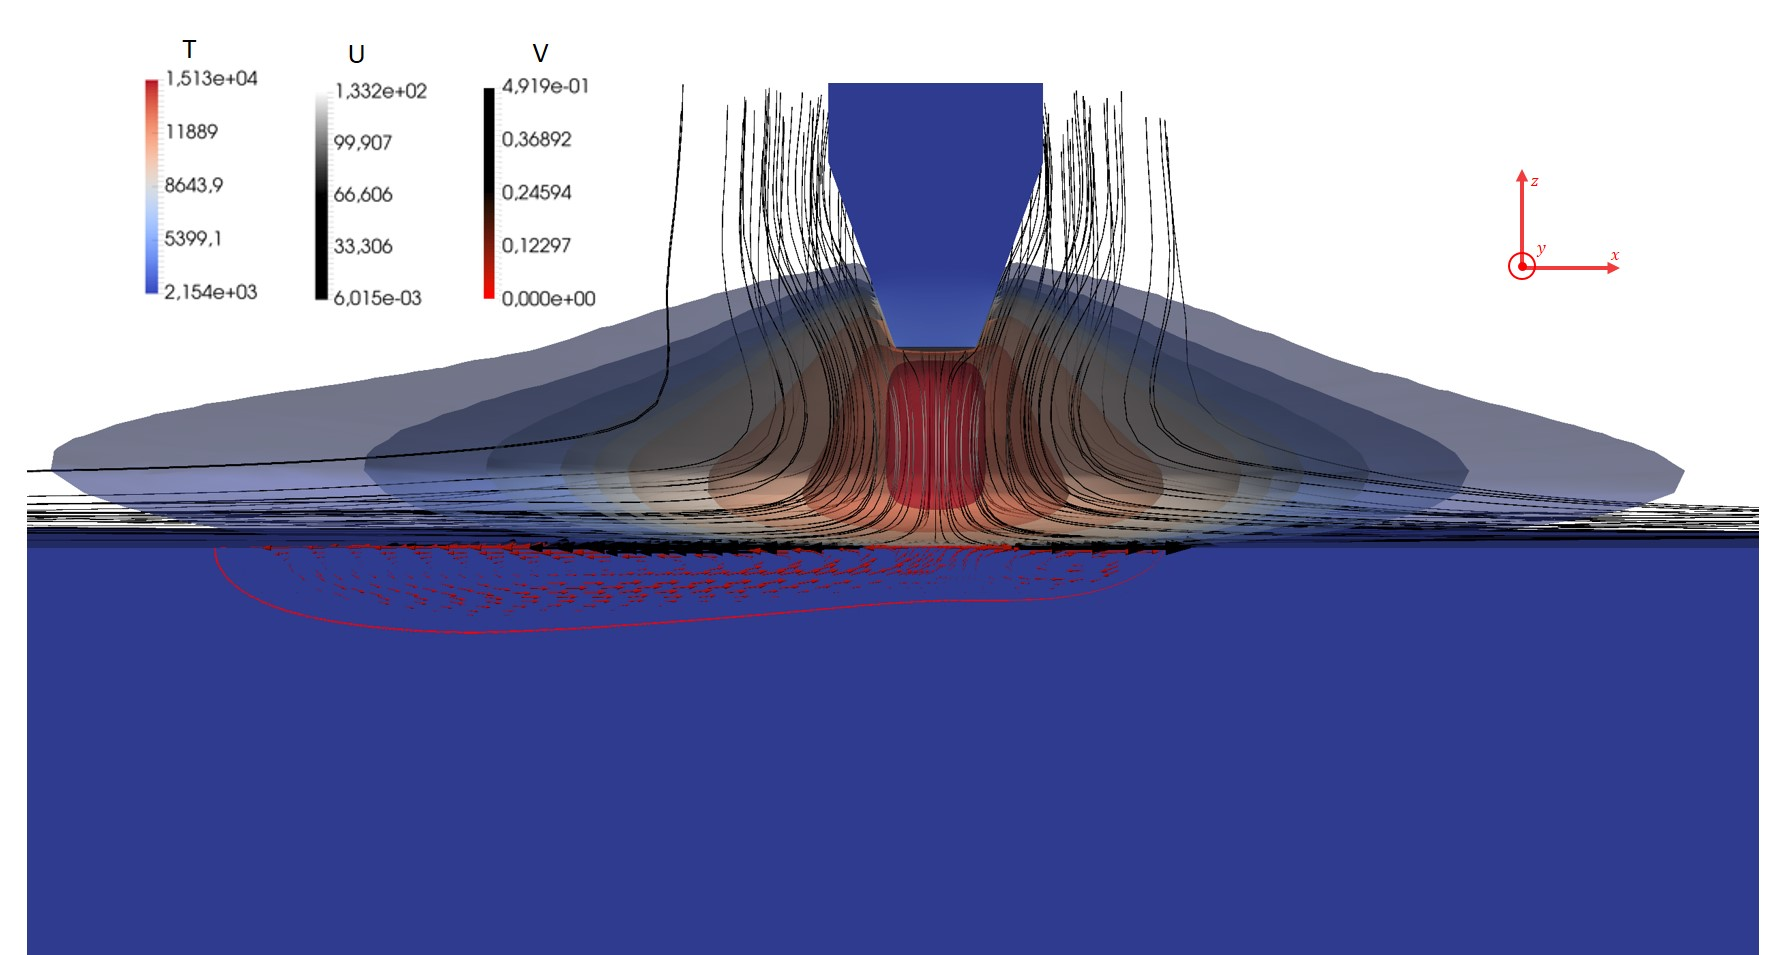
\includegraphics[width=5cm]{images/soudage}\\
          \tiny{\fe{\emph{Simulation magnéto thermo hydrodynamique du soudage TIG (arc plasma + bain) (C. Nahed)}}
                   {\emph{Magneto thermo hydro dynamic simulation of TIG welding (plasma arc + weld pool) (C. Nahed)}}}
        \end{center}
      \end{textblock*}
      }
    \small
    \item<8-> \fe{Magnétostatique}{Magneto-statics}
    \item<8-> \fe{Couplage thermo-hygro-mécanique}{Thermo-hygro-mechanics coupling}
    \item<8-> \fe{Optimisation topologique}{Topology optimization}
    \only<8>{
      \begin{textblock*}{5cm}(6.2cm,-6cm)
        \begin{center}
          \if \animation 1
            \animategraphics[controls,loop,poster=last,width=6cm]{10}{images/topoptim/topoptim.}{001}{100}\\~\\
          \else
            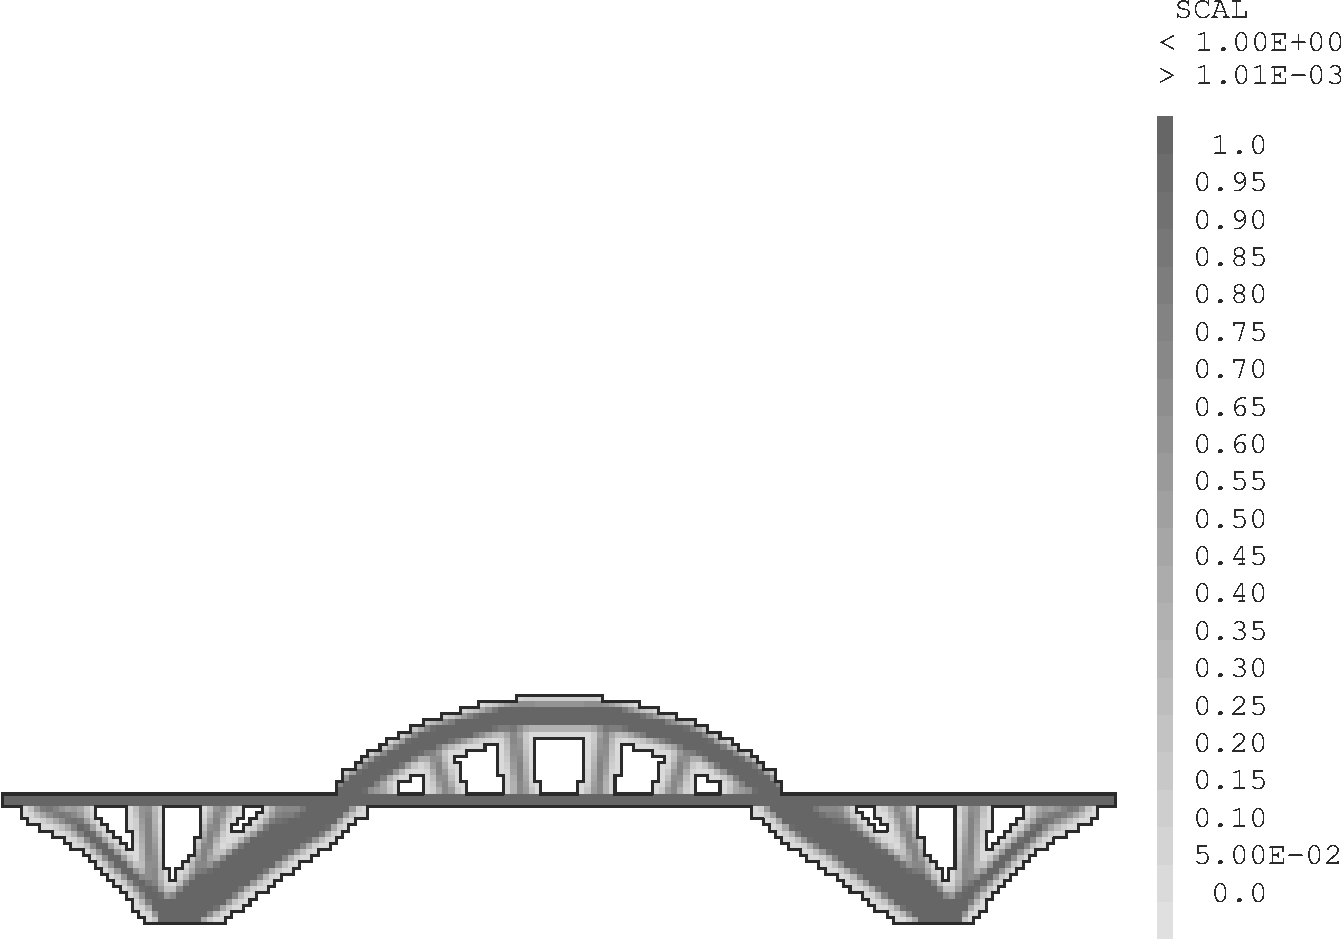
\includegraphics[width=6cm]{images/topoptim/topoptim.100}\\~\\
          \fi
          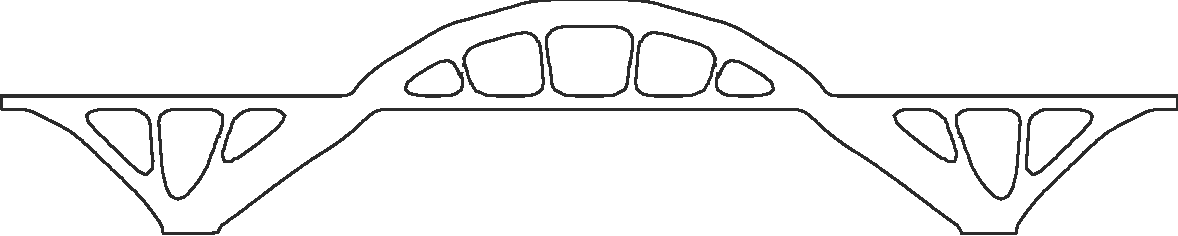
\includegraphics[width=5cm]{images/topoptim/toposurf}\\
          \tiny{\fe{\emph{Optimisation topologique d'un pont}}{\emph{Topology optimization of a bridge}}}
        \end{center}
      \end{textblock*}
      }
  \end{itemize}
\end{frame}

\begin{frame}{\fe{Comment obtenir Cast3M ?}{How to get Cast3M}}
  \begin{itemize}
    \item \fe{Multi plateformes}{Cross platform}\\
    \footnotesize
    \blue{Windows}, \red{Linux}, \green{macOS}
    \normalsize
    \item \fe{Où télécharger Cast3M ?}{Where can I download Cast3M?}\\
    \footnotesize
    \url{https://www-cast3m.cea.fr/index.php?page=dlcastem}
    \normalsize
    \item \fe{Accès au code source}{Access to the source code}\\
    \footnotesize
    \fe{Développement communautaire}{Open collaboration}\\
    \fe{Compilateur / éditeur de liens fournis}{Compiler / Linker are provided}
    \normalsize
    \item \fe{Prix}{Price}\\
    \footnotesize
    \fe{\green{Gratuit} pour la recherche et l'enseignement\\
        \red{Payant} pour une utilisation commerciale}
       {\green{Free} license, for education and research use\\
        \red{Paid} license, for enterprise use}
    \normalsize
    \item \fe{Utilisateurs/clients}{Users/customers}\\
    \footnotesize
    \fe{Universités, écoles d'ingénieurs\\
        IRSN, EDF, SNCF, CNRS, Framatome, Air Liquide, CERN, \dots}
       {Universities, engineering schools\\
        IRSN, EDF, SNCF, CNRS, Framatome, Air Liquide, CERN, \dots}\\
    \scriptsize
    \fe{Outil de référence IRSN pour les analyse de sureté des installations nucléaires françaises\\
        Outil de référence Framatome pour l'analyse en mécanique de la rupture}
       {Reference FEM tool for IRSN for safety analysis of French nuclear installations\\
        Reference tool for Framatome for fracture mechanics}
    \normalsize
    \end{itemize}
\end{frame}

\begin{frame}{\fe{Comment utiliser Cast3M ?}{How to launch Cast3M?}}
  \begin{textblock*}{5cm}(7.9cm,0cm)
    \if \animation 1
      \animategraphics[autoplay,loop,poster=last,width=4.5cm]{10}{images/new_dgibi/new_dgibi-}{000}{235}
    \else
      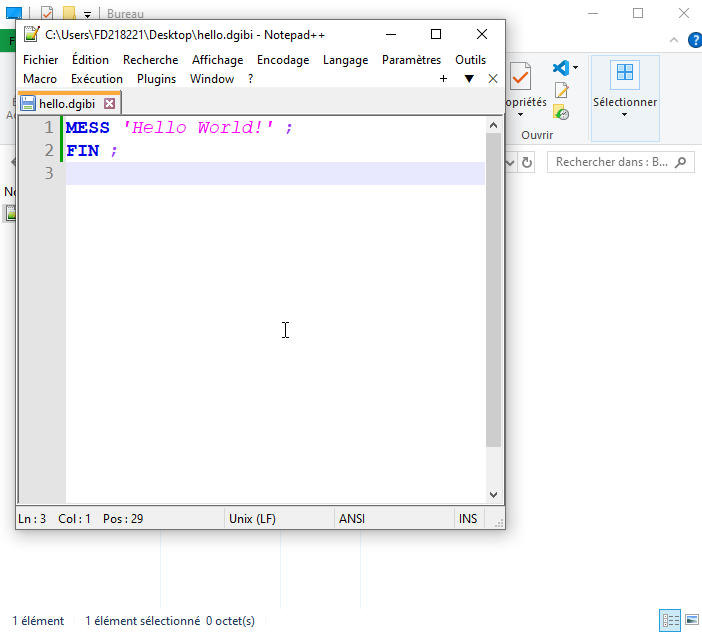
\includegraphics[width=4.5cm]{images/new_dgibi/new_dgibi-235}
    \fi
  \end{textblock*}
  \begin{enumerate}
    \item\fe{Écrire un fichier texte en Gibiane}{Write a Gibiane script in a text file}\\
    \footnotesize
    \fe{et l'enregistrer dans un répertoire de travail}{and save it in a working directory}
    \normalsize
    \item[]\white{O/}\\
    \footnotesize
    \white{et}\\
    \normalsize
    \item[]\white{Cast3M}\\
    \footnotesize
    \white{castem24  hello.dgibi}
    \normalsize
    \item[]\white{U}\\
    \footnotesize
    \white{mode}\\
    \white{castem24}
    \normalsize
  \end{enumerate}
\end{frame}

\begin{frame}{\fe{Comment utiliser Cast3M ?}{How to launch Cast3M?}}
  \begin{textblock*}{5cm}(7.9cm,0cm)
    \if \animation 1
      \animategraphics[autoplay,loop,poster=last,width=4.5cm]{10}{images/new_cmd/new_cmd-}{000}{179}
    \else
      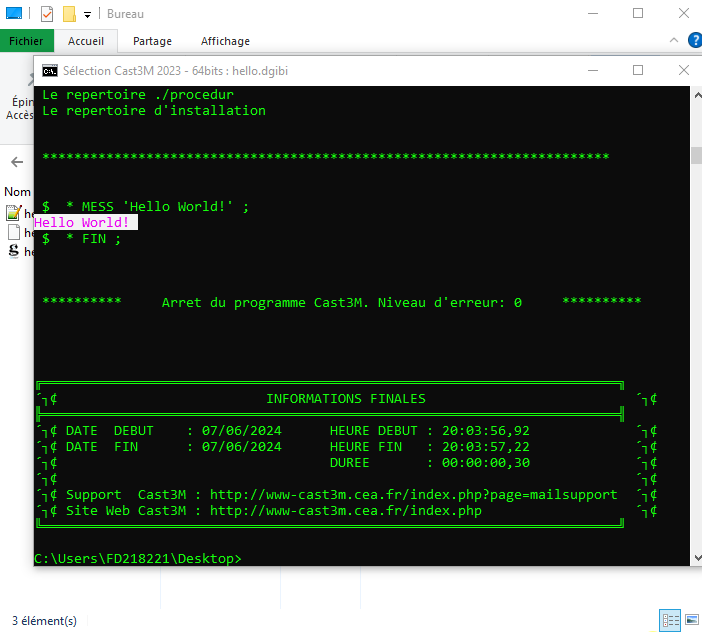
\includegraphics[width=4.5cm]{images/new_cmd/new_cmd-179}
    \fi
  \end{textblock*}
  \begin{enumerate}
    \item\fe{Écrire un fichier texte en Gibiane}{Write a Gibiane script in a text file}\\
    \footnotesize
    \fe{et l'enregistrer dans un répertoire de travail}{and save it in a working directory}
    \normalsize
    \item\fe{Ouvrir un terminal / invite de commandes}{Open a terminal / command prompt}\\
    \footnotesize
    \fe{et se placer dans le répertoire}{and go to the working directory}\\
    \normalsize
    \item\fe{Lancer Cast3M sur ce fichier}{Launch Cast3M on this file}\\
    \footnotesize
    \kwr{castem24 }\kw{ hello.dgibi}
    \normalsize
    \item\fe{Utilisable aussi sans fichier}{Can also be use without file}\\
    \footnotesize
    \fe{mode interactif}{interactive mode}\\
    \kwr{castem24}
    \normalsize
  \end{enumerate}
\end{frame}

\begin{frame}{\fe{Le site web Cast3M}{The Cast3M web site}}
  \begin{center}
    \url{https://www-cast3m.cea.fr/}
  \end{center}
  \begin{itemize}
    \item \fe{Présentation de Cast3M}{Cast3M presentation}
    \item \fe{Formation et tutoriels vidéo}{Training courses and video tutorials}
    \item \fe{Documentation (notices, manuels, sources, exemples)}{Documentation (manual pages, source code, examples)}
    \item \fe{Fiches d'anomalie et de développement}{Anomaly and development reports}
    \item \fe{Téléchargements}{Downloads}
    \item \fe{Contact : support Cast3M}{Contact: Cast3M support}
    \item \fe{Communauté : liste de diffusion, club Cast3M}{Community: mailing list, Cast3M club}
  \end{itemize}
\end{frame}
